\subsection{Data link layer}
Data link layer is the second layer of the \acrshort{osi} reference model. It consists of \acrfull{mac} and \acrfull{llc} layer. The \acrshort{mac} layer is responsible for regulating the access to the shared communication medium among the nodes, while the \acrshort{llc} layer is used to define and control properties of the \acrshort{mac} layer, to shield the upper layers of the model from the physical network and provide inter-operability  across different types of networks. Since the use of \acrshort{llc} layer in practice is limited~\cite{Sohraby2007WirelessApplications}, we will further focus on the \acrshort{mac} layer.

The medium access control layer is responsible for managing the access to the shared communication medium. In wireless networks, it is usually the case that only one device can use the wireless medium at a time, otherwise the interference of wireless signals will render the transmission invalid. The \acrshort{mac} layer resolves this problem, by maintaining a scheme on how and when each node can transmit. The design of the \acrshort{mac} layer is the ``\textit{major determining factor in Wireless Sensor Network performance}''\cite{Sohraby2007WirelessApplications}. 

However, there are several complexities associated with designing this layer. Besides the overall complexity spanning through the whole system, such as limited performance of the devices due to size and power constraints, \acrshort{mac} layer must also account for eventual movement of the devices. Furthermore, when the \acrshort{mac} layer needs to coordinate access to a medium, often the same medium must also be used for this coordination effort. This coordination effort results in better decisions of nodes when to transmit and when not to. The better the decisions, the fewer collisions appear and the less wasted time and transmission power. However, this coordination effort imposes overhead on the communication channel -- on top of the actual data from the sensors, some sort of coordination needs to be added. As~\cite{Sohraby2007WirelessApplications} notes, a trade-off between the quality of the decision and the amount of overhead incurred needs to be made.

There are several metrics that can be used to asses the performance of a \acrshort{mac} layer. 

\begin{table}[htbp]
    \centering
    \begin{tabularx}{\textwidth}{|l|X|p{5em}|}
    \hline
    \textbf{Metrics}&\textbf{Description}&\textbf{Relevance}\\
    \hline
    Delay&Sohraby et. al. defines delay as the amount of time packet spends in the MAC layer before it is transmitted successfully~\cite{Sohraby2007WirelessApplications}.&•\\
    \hline
    Throughput&Throughput is the rate of successful message delivery through the communication channel.&•\\
    \hline
    Scalability&Scalability is the ability of the protocol to maintain its usual performance with increasing amount of devices&•••\\
    \hline
    Stability&Stability is a metrics that measures how well can the system resist changes of the traffic load over a period of time.&•••\\
    \hline
    Fairness&Fairness of a MAC protocol describes how well does the protocol distribute resources among the devices without significantly limiting the throughput.&••\\
    \hline
    \end{tabularx}
    \caption{Comparison of different MAC layer metrics. The \textit{Relevance} column is an approximation of how relevant this metric is in the reefer shipping scenario.}
    \label{tab:mac-metrics}
\end{table}

Generally, the MAC protocols can be divided into two groups: contention-free and contention-based protocols. Contention-free protocols only allow one device to access the medium at the time. This group can be further divided into \textit{fixed assignment} and \textit{dynamic assignment}, depending on how the protocol assigns communication slots to devices. Contention-based protocols allow multiple devices to access the medium at the same time, but provide a recovery mechanism, shall a collision occur. Figure~\ref{fig:mac-categories} displays this grouping.

\begin{figure}[ht]
    \centering
    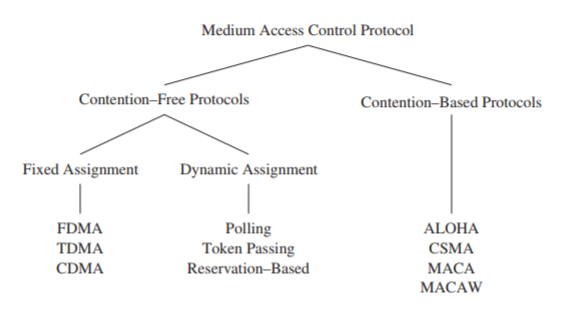
\includegraphics[width=0.8\textwidth]{00images/mac-categories}
    \caption{Categorisation of MAC protocols, according to channel access. Few examples are given for each category. Taken from~\cite{2011MediumControl}.}
    \label{fig:mac-categories}
\end{figure}